%!TEX root = main_RNAPyro_JCB.tex

\section{Methods}
\label{sec:methods}

We introduce a probabilistic model, which aims at capturing both the stability of the folded RNA and its ability to adopt a predefined 3D conformation.
To that purpose, a Boltzmann weighted distribution is used, based on a pseudo-energy function $\PE{\cdot}$ which includes contributions for both the free-energy and its putative isostericity towards a multiple sequence alignment. In this model, the probability that the nucleotide at a given position needs to be mutated (i.e. corresponds to a sequencing error) can be computed using a variant of the \emph{Inside-Outside algorithm}~\cite{Lari1990}.

\subsection{Probabilistic Model}
Let $\Omega$ be an gap-free RNA alignment sequence, $S$ its associated secondary structure, 
then any sequence $s$ has probability proportional to its Boltzmann factor
\begin{align*}
  \mathcal{B}(s) &= e^\frac{-\PE{s}}{RT}, &&\text{with}&\PE{s}&:=\alpha\cdot\ES(s,S)+(1-\alpha)\cdot\EI(s,S,\Omega),
\end{align*}
where $R$ is the Boltzmann constant, $T$ the temperature in Kelvin, $\ES(s)$ and $\EI(s,S,\Omega)$ 
are the free-energy and isostericity contributions respectively (further described below), and $\alpha\in[0,1]$ is an arbitrary parameter that sets the relative weight for both contributions.

\subsubsection{Energy Contribution.}
The free-energy contribution in our pseudo-energy model corresponds to an additive stacking-pairs model, taking values from the Turner 2004 model retrieved from the NNDB~\cite{Turner2010}. Given a candidate sequence $s$ for a secondary structure $S$, the free-energy of $S$ on $s$ is given by
\begin{align*}
  \ES(s,S) = \sum_{\substack{(i,j)\to (i',j')\in S\\ \text{stacking pairs}}}\ES^{\beta}_{s_is_j\to s_{i'}s_{j'}} 
\end{align*}
where $\ES^{\beta}_{ab\to a'b'}$ is set to $0$ if $ab=\varnothing$ (no base-pair to stack onto), the tabulated free-energy of stacking pairs $(ab)/(a'b')$ in the Turner model if available, or $\beta\in[0,\infty]$ for non-Watson-Crick/Wobble entries (i.e. neither $\Gb\Ub$, $\Ub\Gb$, $\Cb\Gb$, $\Gb\Cb$, $\Ab\Ub$ nor $\Ub\Ab$). This latter parameter allows to choose whether to simply penalize invalid base pairs, or forbid them altogether ($\beta = \infty$).
The loss of precision due to this simplification of the Turner model remains reasonable since the targeted secondary structure is fixed 
(e.g. multiloops do not account for base-specific contributions). Furthermore, it greatly eases the design and implementation of dynamic-programming equations. 
\subsubsection{Isostericity Contribution.}
The concept of isostericity score~\cite{Stombaugh2009} is based on the geometric discrepancy (superimposability) of two base-pairs, using individual additive contributions computed by Stombaugh~\emph{et al}~\cite{Stombaugh2009}. Let $s$ be a candidate sequence for a secondary structure $S$, given in the context of a gap-free RNA alignment $\Omega$,  we define the isostericity contribution to the pseudo-energy as
\begin{align*}
  \ES(s,S,\Omega) &= \sum_{\substack{(i,j)\in S\\ \text{pairs}}}\EI^{\Omega}_{(i,j),s_i s_j}, & \text{where}&& 	\EI^{\Omega}_{(i,j),ab}:=
	\frac{
		\sum_{s'\in\Omega}
			\text{\ISO}((s_i',s_j'),(a,b))}
%-		\left(			\text{\ISO}((s_i',s_j'),(s_i,s_j))				\right)	
{		
		|\Omega|
	}
\end{align*}
is the average isostericity of a base-pair in the candidate sequence, compared with the reference alignment.
The $\ISO$ function uses the {Watson-Crick/Watson-Crick} cis isostericity matrix computed by Stombaugh~\emph{et al}~\cite{Stombaugh2009}. Isostericity scores range between $0$ and $9.7$, $0$ corresponding to a perfect isostericity, and a penalty of $10$ is used for missing entries.
The isostericity contribution will favor exponentially sequences that are likely to adopt a similar local conformation as the sequences contained in the alignment.

\subsection{Mutational Profile of Sequences}


Let $s$ be an RNA sequence, $S$ a reference structure, and $m\geq 0$ a desired number of mutations. 
We are interested in  the probability that a given position contains a specific nucleotide, over all sequences having at most $m$ mutations from $s$
%  under the SCFG derivation $S$ 
(formally $\mathbb{P}(s_i = x\mid s,\Omega, S,m)$). 
We define a variant of the
 \emph{Inside-Outside algorithm}~\cite{Lari1990}, allowing us to compute these
 probability. 
%from the two  functions $\mathcal{Z}_*^*$ and $\mathcal{Y}_*^*$. 

The former, defined in Equations~\eqref{eq:Z_in} and~\eqref{eq:Z_rec}, is analogous to the \emph{inside} algorithm.
It is the partition function, i.e. the sum of Boltzmann factors, over all sequences within $[i,j]$, 
knowing that position $i-1$ is composed of nucleotide $a$ (resp. $j+1$ is $b$), within 
$m$ mutations of $s$. The latter, defined by Equations~\eqref{eq:Y_in} and~\eqref{eq:Y_rec},
 computes the \emph{outside} algorithm, i.e.  
the partition function over sequences within $m$ mutations of $s$, restricted to two intervals $[0,i]\cup[j,n-1]$, and 
knowing  that position $i+1$ is composed of $a$ (resp. $j-1$ is $b$). A suitable combination of these terms, given in Equation~\eqref{eq:combine}, gives the total weight, and in turn the probability, of seeing a specific base at a given position.

%Drawing a parallel with stochastic context-free grammars (SCFG), for which the inside-outside algorithm was introduced, the set of sequences can be seen as the language of words having length $n$, generated from a stochastic context-free grammar.
%These rules would limit the number of mutations (i.e. )
% $S$ can be considered as constraining weighing on the shape of parse trees the derivations in a classic 
% of the {SCFG} generating  all  secondary structures of length  $|s|$. 





\subsubsection{Definitions.}
Let $B:=\left\{\Ab,\Cb,\Gb,\Ub\right\}$ be the set of nucleotides.
Given $s\in B^n$ an RNA sequence, let $s_i$ be the nucleotide at position $i$. Let $\Omega$ be a set of un-gapped RNA sequences of
length $n$, and $\Struct$ a secondary structure without pseudoknots. 
\TODOYann{Move above, define secondary structure and add fancy VARNA illustration}

Formally, if $(i,j)$ and $(k,l)$ are base pairs in $S$, there is no overlapping extremities
 $\{i,j\}\cap \{k,l\}=\varnothing$ and either the intersection is empty 
 ($[i,j]\cap[k,l]=\varnothing$) or one is included in the other ($[k,l]\subset[i,j]$ or 
 $[i,j]\subset[k,l])$. 


Let us then remind the Hamming distance function $\delta: B^*\times B^* \to \mathbb{N}^+$, which takes two sequences $s'$ and $s''$ as input, $|s'|=|s''|$, and returns the number of differing positions.
Finally, let us denote by $E_{(i,j),ab \to ab'}^{\Omega,\beta}$ the local contribution of a base-pair $(i,j)$ to the pseudo-energy, such that
\begin{equation}
  E_{(i,j),ab \to a'b'}^{\Omega,\beta}  = \alpha \cdot\ES^\beta_{a b \to a' b'}+(1-\alpha)\cdot\EI^{\Omega}_{(i,j),a'b'}.
\end{equation}
\subsubsection{Inside computation.}
\begin{figure}[t]\centering
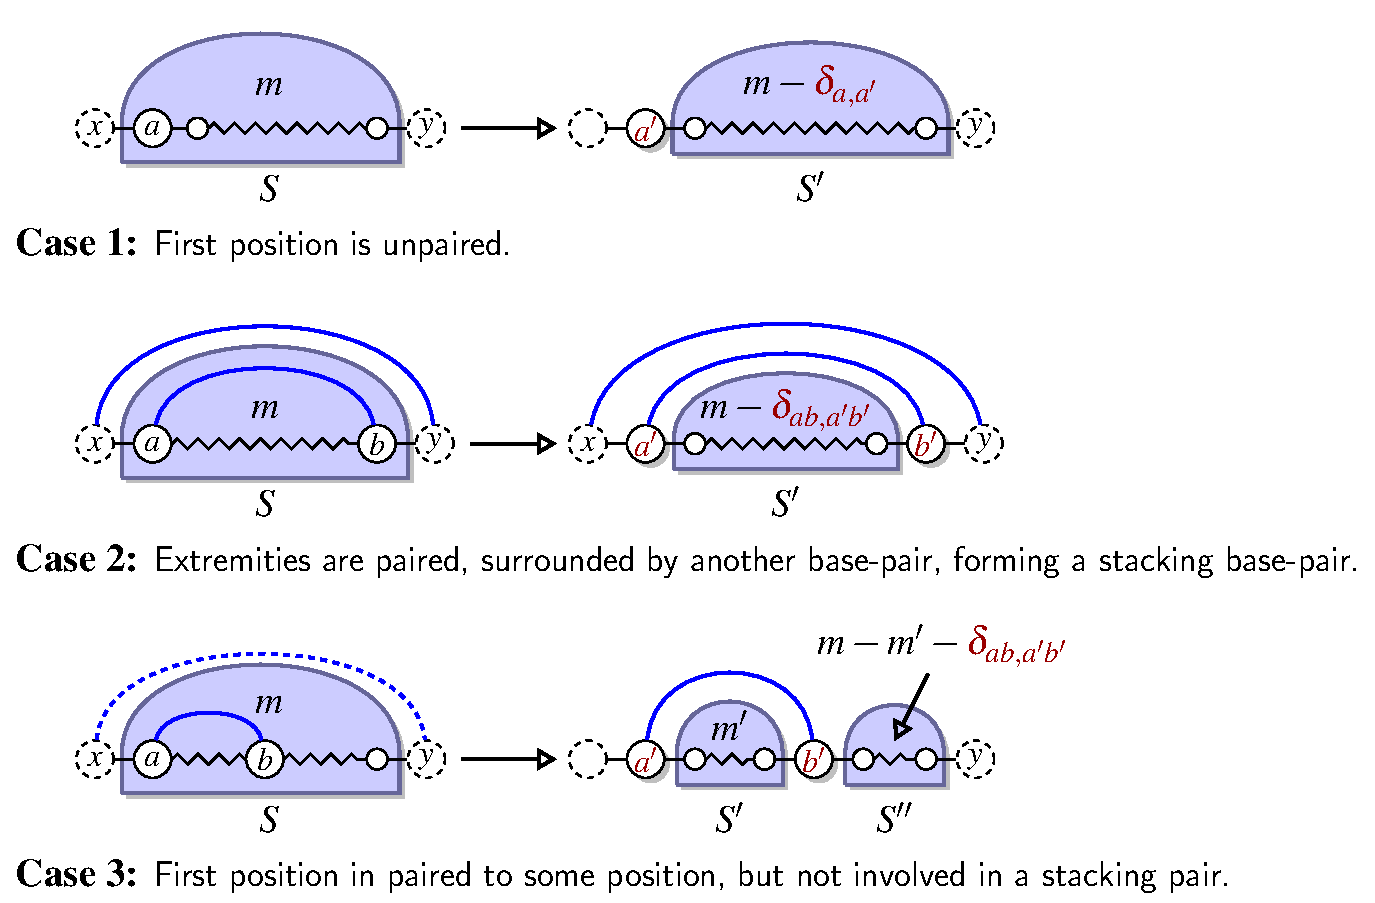
\includegraphics[scale=\ScaleDP]{FigDPInsideWrapper}
\caption{Principle of the inside computation (partition function). Any sequence with mutations  
can be decomposed as a sequence preceded by a, possibly mutated, base 
(Unpaired case), a sequence surrounded by some base-pair (Stacking-pair case), 
or as two sequences segregated by some base-pair (General base-pairing case), and mutations must be distributed between sub-sequences 
and instantiated bases.}
\end{figure}

The \emph{Inside} function $\Z{\Struct}{m}{x,y}$ is simply the partition function, i.e. the sum of Boltzmann factors over all sequences for a substructure $\Struct$, featuring $m$ mutations/errors compared to $s$, and having flanking nucleotides $x$ and $y$. 
\TODOYann{Reformat inside Figure as in Incarnation.}
Such terms can be computed by recurrence, whose initial values are:
\begin{equation}
	\forall x,y\in B\times B, m\in [0,M]:\, \Z{\varepsilon}{m}{x,y}=\left\{
	\begin{array}{ll}
		1 &\text{If } m = 0\\
		0 &\text{Otherwise.}
	\end{array}\right.
\label{eq:Z_in}
\end{equation}
In other words, either there is no sequence at distance $m>0$ of the empty sequence, or the only allowed sequence is the empty sequence ($m=0$), having energy $0$. Since the energetic terms only depend on base pairs, they are not involved in the initial conditions. 
The main recursion itself is composed of four terms:\\

\begin{equation}
\label{eq:Z_rec}
	\Z{i,j}{m}{a,b}:=\left\{
  \begin{array}{ll}
  		\displaystyle
      \sum_{\substack{a'\in \B,\\ \Kron_{a',s_i}\le m}}  
      \Z{i+1,j}{m-\Kron_{a',s_i}}{a',b} &
       \text{[If }S_{i}=-1\text{]}\\
      \displaystyle
      \sum_{\substack{a',b'\in \B^2,\\ \Kron_{a'b',s_is_j}\le m}}
			 e^{\frac{-E_{(i,j),ab \to a'b'}^{\Omega,\beta}}{RT}}
			 \cdot \Z{i+1,j-1}{m-\Kron_{a'b',s_is_j}}{a',b'}&
			 \text{[Else if }S_i=j \land S_{i-1}=j+1\text{]}\\
			 \displaystyle
      \sum_{\substack{a',b'\in \B^2,\\ \Kron_{a'b',s_is_k}\le m}}
      \sum_{m'=0}^{m-\Kron_{a'b',s_is_k}}
   		 e^{\frac{-E_{(i,k),\varnothing\to a'b'}^{\Omega,\beta}}{RT}}
      \cdot\Z{i+1,k-1}{m-\Kron_{a'b',s_is_k}-m'}{a',b'}
      \cdot\Z{k+1,j}{m'}{b',b} &
       \text{[Elif }S_i=k \land i < k \leq j\text{]}\\
      0 \\\text{[Otherwise]}
	\end{array}\right.
\end{equation}
\TODOYann{Rephrase in term of tree, as in Incarnation??}
The cases can be broken down as follows:
\begin{description}
\item[$S_{i}=-1$:] If nucleotide at position $i$ is unpaired, then 
any sequence is a concatenation of a, possibly mutated, nucleotide $a'$ at position  $i$, 
followed by a sequence over $[i+1,j]$ having $m-\Kron_{a',s_i}$ mutations (accounting for a possible mutation 
at position $i$), and having flanking nucleotides $a'$ and $b$.
\item[$S_i=j$ and $S_{i-1}=j+1$:] Any sequence generated in $[i,j]$ consists of two, possibly mutated, nucleotides $a'$ and $b'$, flanking a sequence over $[i+1,j-1]$ having distance $m-\Kron_{a'b',s_is_j}$.
Since positions $i$ and $i-1$ are paired with $j$ and $j+1$ respectively, 
then a stacking energy contribution is added. 
\item[$S_i=k$ and $i<k \leq j$:] If position $i$ is paired and not involved in a stacking, then the 
only term contributing directly to the energy is the isostericity of the base pair $(i,k)$. 
Any sequence on $[i,j]$ consists of two nucleotide $a'$ and $b'$ at positions $i$ and $k$ respectively, flanking a sequence over interval $[i+1,k-1]$ and preceding a (possibly empty) sequence interval $[k+1,j]$. Since the number of mutations sum to $m$ over the whole sequence must , then a parameter $m'$ is introduced to distribute the remaining mutations between the two sequences.
\item[Else:] In any other case, we are in a derivation of the SCFG that does not correspond to the secondary structure $S$, and we return $0$.
\end{description}

\subsubsection{Outside computation.}	
\begin{figure}[t]\centering
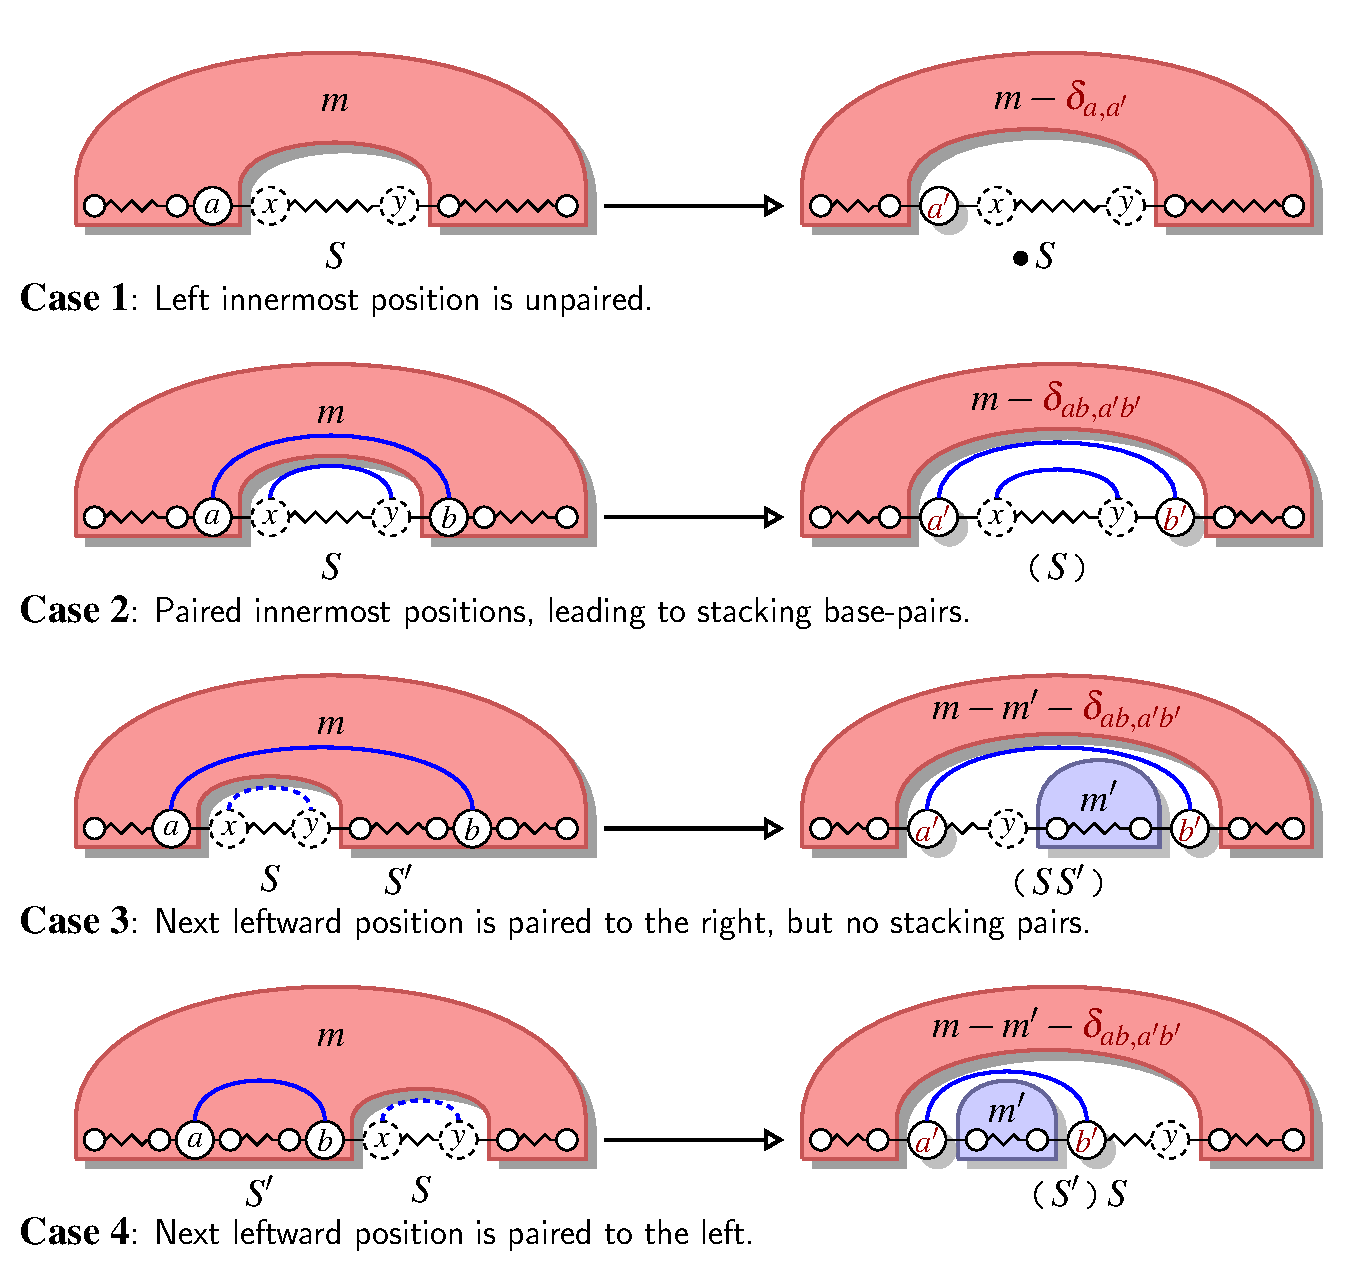
\includegraphics[scale=\ScaleDP]{FigDPOutsideWrapper}
\caption{Principle of the outside computation. Note that the outside algorithm uses intermediate results from the inside algorithm, 
therefore its efficient implementation requires a precomputation of the inside contributions.}
\end{figure}

The \emph{Outside} function, $\mathcal Y$, is the partition function considering only the 
contributions of subsequences $[0,i]\cup[j,n-1]$ over the mutants of $s$ having exactly $m$ mutations between $[0,i]\cup[j,n-1]$ and whose nucleotide at position $i+1$ is $a$ 
(resp. in position $j-1$ it is $b$).
\TODOYann{Reformat outside Figure as in Incarnation.}
The resulting terms $\Y{i,j}{m}{a,b}$ can be computed by recurrence, using as initial conditions:
\begin{equation}
	\Y{-1,j}{m}{X,X}:=
		\displaystyle
	  \Z{j,n-1}{m}{X,X}.
\label{eq:Y_in}
\end{equation}
The recurrence below extends the interval $[i,j]$, by including $i-1$ when
position $i$ not base paired, or extended in both directions if $i$ is paired with a position $k>j$.
% Thus, when we need
%to evaluate an interval as $(-1,j)$, all stems between $(0,j)$ are taken into account and the
%structure between $(j,n-1)$ must be a set of independent stems. Therefore,
% all the outside energy between $[j,n-1]$ is
%equal to $\Z{j,n-1}{m}{X,X}$, for any $X\in B$. 
The recursion itself unfolds as follows:
\begin{equation}
\resizebox{\textwidth}{!}{%
	$\Y{i,j}{m}{a,b} = \left\{
  \begin{array}{ll}
		\displaystyle
    \sum_{\substack{a'\in \B,\\ \Kron_{a',s_i}\le m}}
    \Y{i-1,j}{m- \Kron_{a',s_i}}{a',b} &
    \text{Elif }S_i=-1 \\
    \displaystyle
    \sum_{\substack{a'b'\in \B^2,\\ \Kron_{a'b',s_is_j}\le m}}
		 e^{\frac{-E_{(i,j),ab \to a'b'}^{\Omega,\beta}}{RT}}\cdot
    \Y{i-1,j+1}{m- \Kron_{a'b',s_is_j}}{a',b'} &
   	 \text{Elif }S_{i}=j \land S_{i+1}=j-1\\
		 \displaystyle
		 \sum_{\substack{a'b'\in \B^2,\\ \Kron_{a'b',s_is_k}\le m}}
		 \sum_{m'=0}^{m-\Kron_{a'b',s_is_k}}
  		 e^{\frac{-E_{(i,k),\varnothing\to a'b'}^{\Omega,\beta}}{RT}}
		 \cdot\Y{i-1,k+1}{m- \Kron_{a'b',s_is_k} - m'}{a',b'}
     \cdot\Z{j,k-1}{m'}{b,b'} &
		 \text{Elif }S_{i}=k \geq j\\
		 \displaystyle
		 \sum_{\substack{a'b'\in \B^2,\\ \Kron_{a'b',s_ks_i}\le m}}
		 \sum_{m'=0}^{m-\Kron_{a'b',s_ks_i}}
   	 e^{\frac{-E_{(k,i),\varnothing\to a'b'}^{\Omega,\beta}}{RT}}
		 \cdot\Y{k-1,j}{m- \Kron_{a'b',s_ks_i} - m'}{a',b}
     \cdot\Z{k+1,i-1}{m'}{a',b'} &
		 \text{Elif }-1 < S_{i}=k < i\\
		 0 & \text{Otherwise}
  \end{array}\right.$
}\label{eq:Y_rec}
\end{equation}
\TODOYann{Rephrase in term of tree, as in Incarnation??}
The five cases can be broked down as follows.
\begin{description}
\item[$S_i=-1$:] If the nucleotide at position $i$ is not paired, then the value is the same
as if we decrease the lower interval bound by $1$ (i.e. $i-1$), and consider all possible
nucleotides $a'$ at position $i$, correcting the number of mutants
in function of $\Kron_{a',s_i}$.
\item[$S_{i}=j$ and $S_{i+1}=j-1$:] If nucleotide $i$ is paired with $j$ and nucleotide $i+1$ is
paired with $j-11$, we are in the only case were stacked base pairs can occur. We thus add
the energy of the stacking and of the isostericity of the base pair $(i,j)$. What is left
to compute is the \emph{outside} value for the interval $[i-1,j+1]$ over all possible nucleotides 
$a',b'\in B^2$ at positions $i$ and $j$ respectively.
\item[$S_{i}=k \geq j$:]If nucleotide $i$ is paired with position $k\geq j$, 
and is not stacked inside, the 
only term contributing directly to the energy is the isostericity of base pair $(i,k)$. 
Therefore, we consider the outside interval $[i-1,k+1]$, multiplying it by the \emph{inside}
value of the newly included interval (i.e. $[j,k-1]$), for 
all possible values $a',b'\in B^2$ for nucleotides at positions $i$ and $k$ respectively.
\item[$-1<S_{i}<i$:]As above but if position $i$ is paired with a lower value.
\item[Else:] Any other derivation of the SCFG does not correspond to the 
secondary structure $S$, and we return $0$.


\end{description}

\subsubsection{Combining Inside and Outside Values into Point-Wise Mutations Probabilities.}
By construction, the partition function over all sequences at exactly $m$ mutations of a reference sequence $s$ can 
be either described from the \emph{inside} contribution $\Z{0,n-1}{m}{X,X}$ of the whole sequence,
$\forall X\in B$, or from \emph{outside} terms as:
$$
	\Z{0,n-1}{m}{X,X}
	\equiv
	\sum_{\substack{a\in \B,\\ \Kron_{a,s[k]}\le m}}	
	\Y{k-1,k+1}{m-\Kron_{a,s[k]}}{a,a},\forall k \text{	unpaired.}
$$

We are now left to compute the probability that a given position is a given nucleotide.
We leverage the \emph{Inside-Outside} construction to immediately obtain the following $3$ cases.
Given $i\in[0,n-1],x\in B$, and $M\geq 0$ a bound on the number of allowed mutations, one defines
\begin{equation}
	\mathbb{P}(s_i = x\;|\; M) := \frac{\mathcal{W}^M_{\substack{i, [x]}}}{\sum_{m=0}^{M}\Z{0,n-1}{m}{X,X}}\label{eq:normalize}
\end{equation}
where $\mathcal{W}{\substack{\ast\\ \ast}}$ is defined by:
\begin{equation}
\resizebox{\textwidth}{!}{%
$ \mathcal{W}^M_{\substack{i, [x]}} =  \left\{
	\begin{array}{ll}
			\sum_{m=0}^{M}
			\Y{i-1,i+1}{m-\Kron_{x,s_i}}{x,x}
		&\text{If }S_i = -1\\
			\displaystyle
			\sum_{m=0}^{M}
			\sum_{\substack{b\in B\\\Kron_{xb,s_is_k\leq m}}}
			\sum_{m'=0}^{m-\Kron_{xb,s_is_k}}
     	 e^{\frac{-E_{(i,k),\varnothing\to xb}^{\Omega,\beta} }{RT}}
			\cdot\Y{i-1,k+1}{m-\Kron_{xb,s_is_k-m'}}{x,b}
			\cdot\Z{i+1,k-1}{m'}{x,b}
		&\text{If }S_i=k>i\\
    \displaystyle
			\sum_{m=0}^{M}
			\sum_{\substack{b\in B\\\Kron_{bx,s_ks_i\leq m}}}
			\sum_{m'=0}^{m-\Kron_{bx,s_ks_i}}
     	 e^{\frac{-E^{\Omega, \beta}_{(k,i),\varnothing\to bx}}{RT}}
			\cdot\Y{k-1,i+1}{m-\Kron_{bx,s_ks_i-m'}}{b,x}
			\cdot\Z{k+1,i-1}{m'}{b,x}
		&\text{If }S_i=k<i
	\end{array}\right.
$}\label{eq:combine}
\end{equation}

\TODOYann{Rephrase as tree constructs}
\TODOVlad{Add illustration of Inside/Outside combination (adapted from RECOMB presentation??)}
In every case, the denominator is the sum of the partitions function of exactly $m$ mutations, 
for $m$ smaller or equal to our target $M$. The numerators are divided in the following three cases.
\begin{description}
\item[$S_i=-1$:] If the nucleotide at position $i$ is not paired, we are concerned by the weights
over all sequences which have at position $i$ nucleotide $x$, which is exactly the sum
of the values of $\Y{i-1,i+1}{m-\Kron_{x,s_i}}{x,x}$, for all $m$ between $0$ and $M$.
\item[$S_i=k>i$:] Since we need to respect the derivation of the secondary structure $S$, if 
position $i$ is paired, we must consider the two partition functions. The \emph{outside} of the 
base pair, and the \emph{inside}, for all possible values for the nucleotide at position $k$, and
all possible distribution of the mutant positions between the inside and outside of the base pair. We also add the term of isostericity for this specific base pair.
\item[$S_i=k<i$:] Same as above, but with position $i$ pairing with a lower position.
\end{description}

\subsection{Complexity Considerations}
Equations~\eqref{eq:Z_rec} and~\eqref{eq:Y_rec} can be computed using dynamic programming. Namely, the $\mathcal{Z}^{*}_{*}$ and $\mathcal{Y}^{*}_{*}$ terms are computed starting from smaller values of $m$ and interval lengths, memorizing the results as they become available to ensure constant-time access during later stages of the computation. Furthermore, energy terms $E(\cdot)$ can be accessed in constant time thanks to a simple precomputation (not described)  of the isostericity contributions in $\Theta(n\cdot|\Omega|)$. Computing any given term therefore requires $\Theta(m)$ operations.

In principle, $\Theta(m\cdot n^2)$ terms, identified by $(m,i,j)$ triplets, should be computed.
However, a close inspection of the recurrences reveals that the computation can be safely restricted to a subset of intervals $(i,j)$.
For instance, the inside algorithm only requires computing intervals $[i,j]$ that do not break any base-pair, and whose next position $j+1$ is either past the end of the sequence, or is base-paired prior to $i$. Similar constraints hold for the outside computation, resulting in a drastic limitation of the combinatorics of required computations, dropping from $\Theta(n^2)$ to $\Theta(n)$ the number of terms that need to be computed and stored. Consequently the overall complexity of the algorithm is $\Theta(n\cdot(|\Omega|+m^2))$ arithmetic operations and $\Theta(n\cdot(|\Omega|+m))$ memory.
